\subsection{Faust - Processing Layer} \label{sec:faust}

\subsubsection{Introduzione}
Per soddisfare il requisito opzionale del calcolo del punteggio di salute, si è scelto di utilizzare Faust, una libreria \textit{Python}\textsubscript{\textit{G}} ispirata al modello di \textit{Kafka}\textsubscript{\textit{G}}\textsubscript{\textit{G}} Streams.

Faust facilita l'elaborazione di flussi di dati distribuiti in tempo reale, rendendola una libreria ideale per questo caso d'uso.
Offre un'interfaccia di alto livello che astrae le complessità di \textit{Kafka}\textsubscript{\textit{G}}\textsubscript{\textit{G}}, rendendo la raccolta dati semplice e intuitiva.
Inoltre Faust è progettato per essere scalabile e può essere utilizzato per gestire grandi volumi di dati.

\paragraph{Faust \& Schema Registry} 
Faust deserializza i messaggi dei topic in conformità allo schema definito nello Schema Registry. Qualora si riscontrino messaggi non conformi, essi vengono eliminati. I messaggi validi vengono successivamente processati e instradati verso un topic \textit{Kafka}\textsubscript{\textit{G}} dedicato.

La gestione della connessione allo Schema Registry è integrata in Faust. Dopo aver fornito l'indirizzo dello Schema Registry nella configurazione dell'applicazione Faust, essa si occupa di validare i messaggi in base allo schema registrato per il relativo topic.

\paragraph{Calcolo del punteggio di salute}
Il punteggio di salute rappresenta un indicatore sintetico del benessere generale di una città, viene calcolato sulla base di tre tipologie di misurazioni:
\begin{itemize}
    \item Temperatura;
    \item Umidità;
    \item Livello di polveri sottili nell'aria (PM10).
\end{itemize}

Il calcolo del punteggio di salute avviene in due fasi:
\begin{enumerate}
    \item \textbf{Incrementi:} 
    \begin{itemize}
        \item A intervalli regolari, per ciascuna tipoligia di misurazione, viene calcolato un incremento basato sulle sole misurazioni acquisite all'interno dell'intervallo;
        \item Ciascuna tipologia di misurazione ha un suo algoritmo di calcolo dell'incremento, basato su soglie predefinite di benessere.
    \end{itemize}
    \item \textbf{Punteggio Finale:}
    \begin{itemize}
        \item Il punteggio di salute finale si ottiene sommando gli incrementi calcolati per le tre tipologie di misurazioni;
        \item Punteggi più alti indicano un minore stato di benessere, con la necessità di interventi per migliorare la qualità della vita.
    \end{itemize}
\end{enumerate}

\subsubsection{Componenti Faust \& Processing Layer}
\begin{itemize}
    \item \textbf{Applicazione Faust:}
    \begin{lstlisting}[style=code]
    faust.App(<nome_app>, \textit{broker}\textsubscript{\textit{G}}=<broker_kafka>)
    \end{lstlisting} 
    \begin{itemize}
        \item Un'applicazione Faust è un \textit{programma}\textsubscript{\textit{G}} \textit{Python}\textsubscript{\textit{G}} che elabora flussi di dati in tempo reale da \textit{Kafka}\textsubscript{\textit{G}}\textsubscript{\textit{G}};
        \item \textbf{nome\_app:} Identifica l'applicazione, coincide con il \textit{ConsumerGroup} di \textit{Kafka}\textsubscript{\textit{G}};
        \item \textbf{broker\_kafka:} Indirizzo del \textit{broker}\textsubscript{\textit{G}} \textit{Kafka}\textsubscript{\textit{G}}\textsubscript{\textit{G}} (hostname: porta);
        \item Importante configurare l'applicazione con l'indirizzo dello Schema Registry per garantire la validazione e deserializzazione dei messaggi.
    \end{itemize}

    \item \textbf{Topic:}
    \begin{lstlisting}[style=code]
    app.topic(<nome_topic>, value_type=<tipo_dato>)
    \end{lstlisting}  
    \begin{itemize}
        \item \textbf{nome\_topic:} Nome del topic \textit{Kafka}\textsubscript{\textit{G}}\textsubscript{\textit{G}} a cui iscrivere l'app Faust;
        \item \textbf{tipo\_dato:} Classe che rappresenta il tipo di dato del topic (es. faust\_measurement);
        \item Nel caso si vogliano aggiungere altri topic da cui consumare dati basterà aggiungerli prima del parametro value\_type separati da virgole.
    \end{itemize}

    \item \textbf{Tipo di dato atteso:}
     \begin{lstlisting}[style=code]
    class faust\_measurement(faust.Record, serializer='\textit{json}\textsubscript{\textit{G}}')
    \end{lstlisting}  
    \begin{itemize}
        \item È una classe che eredita da \textbf{faust.Record};
        \item \textbf{faust.Record} è una classe fornita dalla libreria Faust che semplifica la definizione di record per la rappresentazione dei dati in streaming;
        \item Rappresenta una singola misurazione proveniente da un \textit{sensore}\textsubscript{\textit{G}}. Viene usata nella applicazione Faust per definire il tipo di dati atteso nei topic \textit{Kafka}\textsubscript{\textit{G}}\textsubscript{\textit{G}}.
    \end{itemize}

    \item \textbf{Modello per il calcolo del punteggio di salute:}
    \begin{itemize}
        \item \textbf{Processore di misurazioni:}
        Tramite il \textit{pattern}\textsubscript{\textit{G}} \textit{Object Adapter} e l'interfaccia \textit{processor} l'app Faust invia le misurazioni ottenute dai topic al modello per il calcolo del punteggio di salute che verrà adattato come \textit{processor}.
    \end{itemize}

    \item \textbf{Agente di elaborazione:} 
    \begin{lstlisting}[style=code]
    @app.agent(<topic>)
    \end{lstlisting}  
    \begin{itemize}
        \item Permette di definire una funzione asincrona che elabora i dati dai topic;
        \item La funzione riceve un iteratore di oggetti del tipo specificato per il topic;
        \item La funzione esegue l'elaborazione desiderata su ogni misurazione.
    \end{itemize}

    \item \textbf{Interfaccia \textit{processor}:}
    \begin{itemize}
        \item Viene utilizzata per definire un contratto di logiche di elaborazione;
        \item Viene utilizzata dagli agenti di elaborazione per inviare le misurazioni al modello per il calcolo del punteggio di salute.
    \end{itemize}

    \item \textbf{Task aggiuntivo} (opzionale): 
    \begin{lstlisting}[style=code]
    @app.task()
        \end{lstlisting}  
    \begin{itemize}
        \item Definisce una funzione eseguita una sola volta all'avvio dell'applicazione;
        \item Nel nostro progetto, viene chiamato il metodo \textit{start()} del thread adibito all'ottenimento e scrittura periodico dei punteggi di salute.
    \end{itemize}
\end{itemize}

\subsubsection{Processing layer data-flow}
Di seguito esposto il flusso dei dati per il calcolo del punteggio di salute.

\begin{figure}[H]
    \centering
    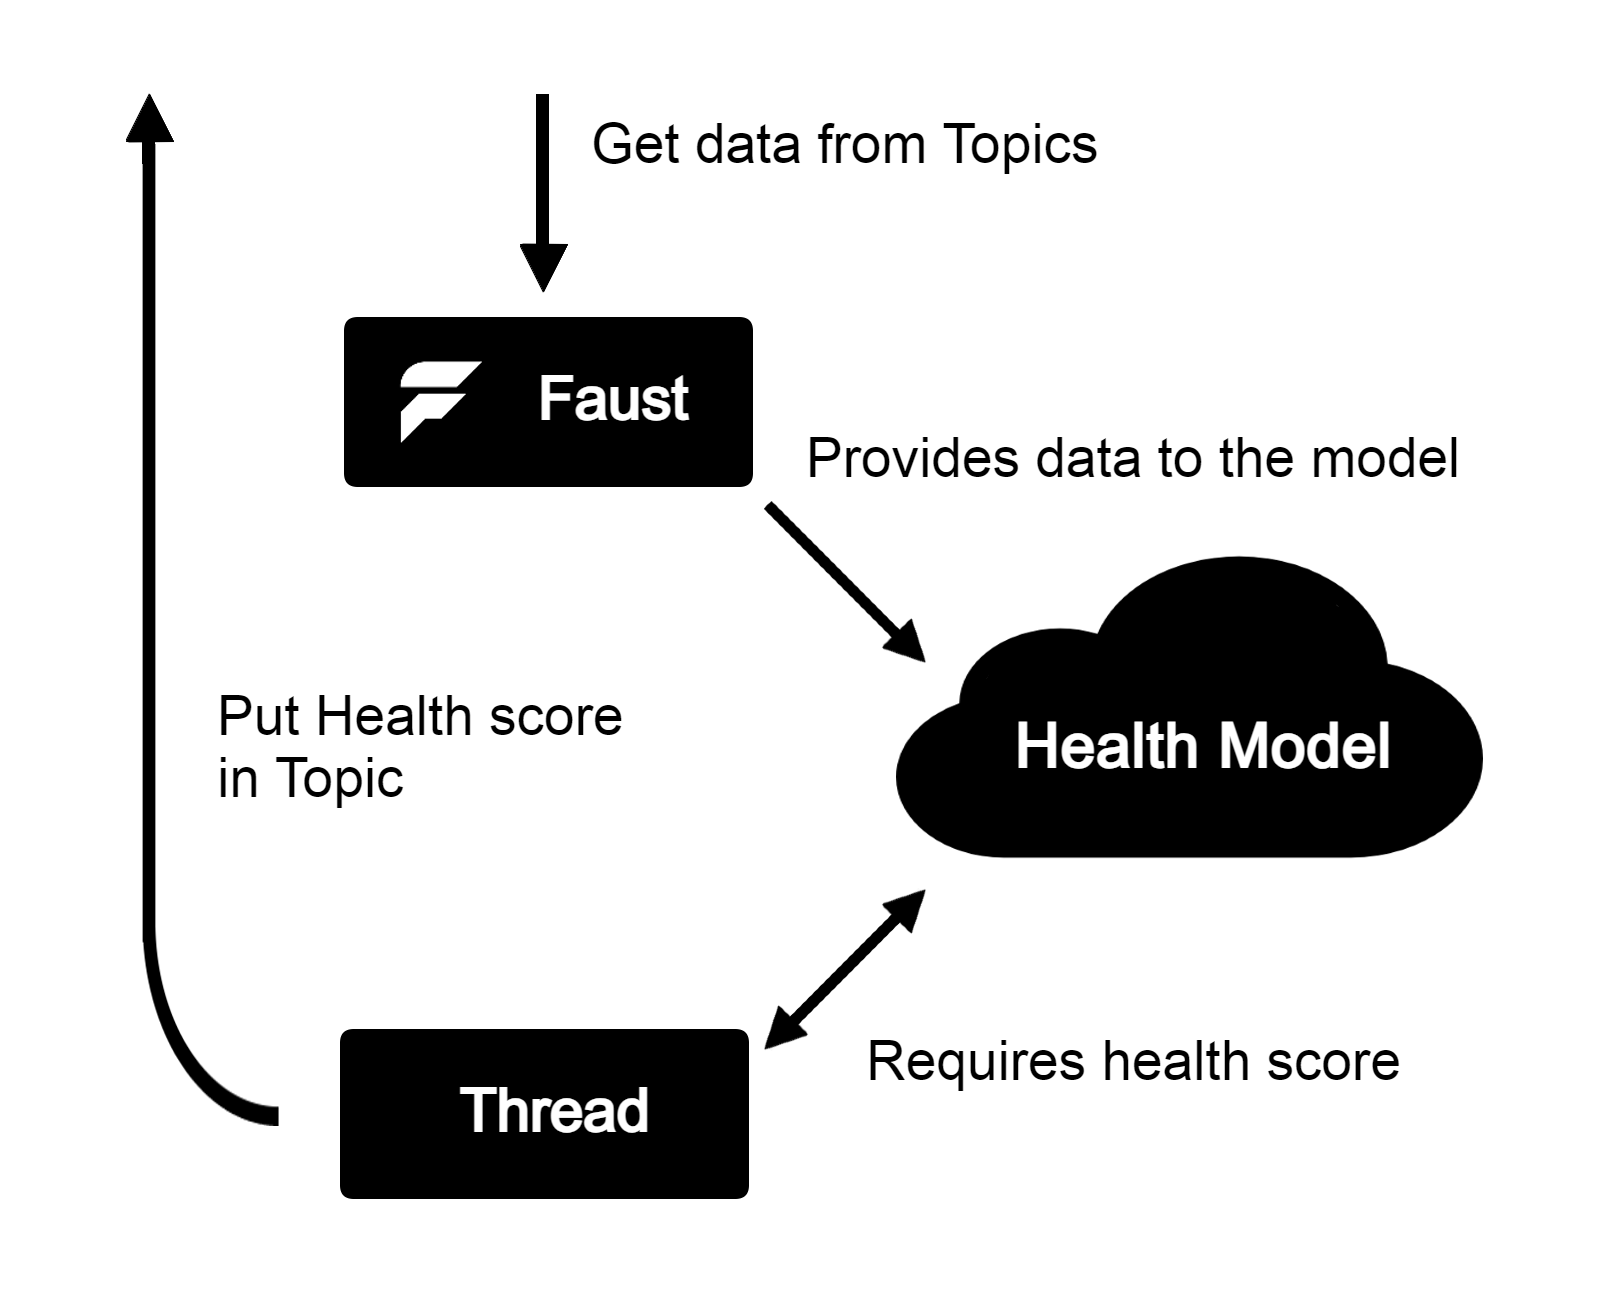
\includegraphics[width=0.8\textwidth]{../Images/SpecificaTecnica/faustFlow.png}
    \caption{Faust data-flow}
    \label{fig: FaustDataflow}
\end{figure}
In breve:
\begin{enumerate}
    \item Faust ottiene le misurazioni dai topic;
    \item Tramite una porta di accesso le fornisce al modello per il calcolo del punteggio di salute;
    \item Quando l'applicazione Faust viene avviata questa avvia a sua volta un Thread che periodicamente ottiene i punteggi di salute calcolati sulla base delle misurazioni ottenute da Faust e tramite il modulo Writer li invia al topic \textit{Kafka}\textsubscript{\textit{G}} dedicato.
\end{enumerate}

\subsubsection{Modello per il calcolo del punteggio di salute}
\begin{figure}[H]
    \centering
    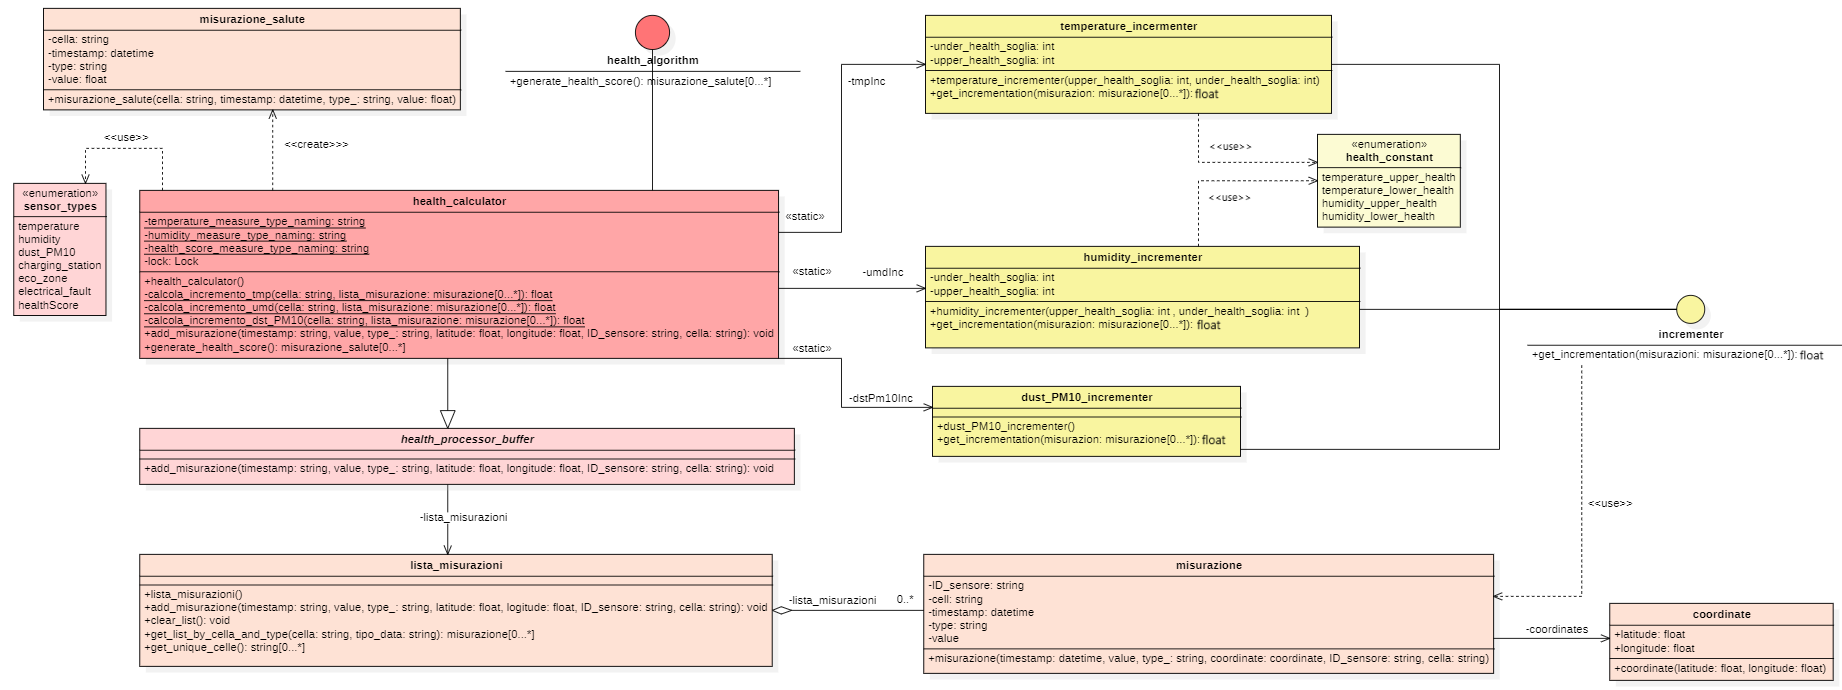
\includegraphics[width=1\textwidth]{../Images/SpecificaTecnica/healthModel.PNG}
    \caption{Modello per il calcolo del punteggio di salute - InnovaCity}
    \label{fig: healthModello}
\end{figure}

Il modello per il calcolo del punteggio di salute riceve le letture dei sensori attraverso gli agenti di elaborazione dell'applicazione Faust, i quali sono in ascolto sui topic \textit{Kafka}\textsubscript{\textit{G}}\textsubscript{\textit{G}} relativi alle misurazioni di temperatura, umidità e polveri sottili PM10.

Ad intervalli regolari, il \textit{sistema}\textsubscript{\textit{G}} calcola il punteggio di salute della città basandosi su tali misurazioni. Una volta effettuato il calcolo, il risultato è reso disponibile in un topic \textit{Kafka}\textsubscript{\textit{G}}\textsubscript{\textit{G}} dedicato.
Il modello che racchiude la logica per il calcolo, richiamato a intervalli regolari, è quello attualmente preso in esame.

In sintesi, il modello:
\begin{itemize}
    \item Riceve le misurazioni di temperatura, umidità e polveri sottili dall'agente dell'app Faust;
    \item Riceve da un thread la richiesta ad intervalli regolari di calcolare i punteggi di salute per le celle della città con le misurazioni ottenute in tempo reale.
\end{itemize}

In modo simile a quanto accade in un'\textit{architettura}\textsubscript{\textit{G}} esagonale, la logica del modello è completamente disaccoppiata dai suoi utilizzatori, i quali interagiscono con esso tramite specifiche classi adapter. Questo approccio promuove la separazione delle preoccupazioni e favorisce la modularità del \textit{sistema}\textsubscript{\textit{G}}. Gli adapter fungono da ponte tra il modello e gli utilizzatori, consentendo una comunicazione fluida e senza dipendenze dirette. Così, eventuali cambiamenti nella logica del modello possono essere implementati senza influenzare gli utilizzatori, garantendo una maggiore flessibilità e manutenibilità del \textit{sistema}\textsubscript{\textit{G}} nel suo complesso.

Il presente modulo è concepito per fornire la logica relativa al puro calcolo del punteggio di salute della città. Tale calcolo si basa su un modello che tiene conto delle misurazioni sopra citate ed è stato progettato al fine di determinare un punteggio di salute per ciascuna cella della città in cui sono presenti misurazioni delle suddette tipologie.

\paragraph{Design pattern Strategy}

Il modello per il calcolo del punteggio di salute è stato ideato mediante l'utilizzo del design \textit{pattern}\textsubscript{\textit{G}} Strategy. Tale \textit{pattern}\textsubscript{\textit{G}} consente di definire una famiglia di algoritmi, di incapsularli e renderli intercambiabili. Ciò permette di variare l'algoritmo impiegato per il calcolo del punteggio di salute senza incidere sui suoi utilizzatori. In particolare, l'interfaccia \textit{health\_algorithm} stabilisce il contratto che deve essere rispettato da tutti gli algoritmi per il calcolo del punteggio di salute.

Inoltre, un'implementazione del \textit{pattern}\textsubscript{\textit{G}} \textit{Strategy} è presente anche negli "Incrementers". Questi, a partire dalle misurazioni fornite, restituiscono un valore da sommare al punteggio di salute della città. Tale incremento è determinato in base a delle soglie predefinite di temperatura, umidità e polveri sottili PM10, le quali sono definite di default in \textit{health\_constants} ma possono essere impostate al momento della costruzione.

In particolare, l'interfaccia \textit{incrementer} specifica il contratto che deve essere rispettato da tutti gli Incrementers. Vengono implementati tre Incrementers, uno per la temperatura, uno per l'umidità e uno per le polveri sottili PM10, come strategie del \textit{pattern}\textsubscript{\textit{G}} Strategy.

\paragraph{Classi, interfacce, metodi e attributi}
\begin{itemize}
    \item{\textbf{Interfaccia: \textit{health\_algorithm}}}
    \begin{itemize}
    \item \textbf{Metodi:}
    \begin{itemize}
        \item \textbf{generate\_new\_health\_score(): List[misurazione\_salute] [abstractmethod]} - Un metodo astratto che, nelle sue implementezioni concrete genera un punteggio di salute.
    \end{itemize}
    \item\textbf{Note:}
        \begin{itemize}
            \item L'interfaccia definisce il contratto per un algoritmo di calcolo per un punteggio di salute. Le sottoclassi devono implementare il metodo \textit{generate\_new\_health\_score()};
            \item Rappresenta la componente "Strategy" del \textit{pattern}\textsubscript{\textit{G}} omonimo;
            \item Per rispettare il Single Responsibility Principle \textit{(SRP)}, \textit{health\_algorithm} è stata divisa dalla logica di buffering delle misurazioni presente nella classe astratta \textit{health\_processor\_buffer} poiché l'utilizzatore \textit{health\_calculator\_thread} non utilizza i metodi per il buffering.
        \end{itemize}
    \end{itemize}

    \item\textbf{Classe astratta: \textit{health\_processor\_buffer}}
    \begin{itemize}
    \item\textbf{Attributi:}
        \begin{itemize}
        \item \textbf{lista\_misurazioni: lista\_misurazioni [private]} - Una lista di oggetti \textit{misurazione};
        \item \textbf{lock: threading.Lock [private]} - Un oggetto lock per gestire l'accesso concorrente alla lista di misurazioni.
    \end{itemize}
    \item \textbf{Metodi:}
    \begin{itemize}
        \item \textbf{add\_misurazione(timestamp, value, type\_, latitude, longitude, ID\_sensore, cella): None [public]} - Aggiunge una nuova misurazione alla lista di misurazioni;
        \item \textbf{clear\_list(): None [public]} - Svuota la lista di misurazioni.
    \end{itemize}
    \item\textbf{Note:}
        \begin{itemize}
            \item La classe astratta definisce un buffer di misurazioni per effettuare processing su di esse;
            \item La logica di buffering e quella dell'algoritmo per il calcolo del punteggio di salute vengono separate in due astrazioni per rispettare il Single Responsibility Principle \textit{(SRP)}. Gli utilizzatori di questa classe, ovvero i Processor, sono interessati esclusivamente al metodo per l'invio del dato al buffer;
            \item La classe astratta definisce un'interfaccia per la comunicazione con gli utilizzatori esterni al modello.
        \end{itemize}
    \end{itemize}
    \item{\textbf{Classe: \textit{health\_calculator}}}
    \begin{itemize}
    \item\textbf{Attributi:}
        \begin{itemize}
        \item \textbf{tmpInc: temperature\_incrementer [private]} - Utilizzato per il calcolo dell'incremento di temperatura;
        \item \textbf{umdInc: humidity\_incrementer [private]}; - Utilizzato per il calcolo dell'incremento di umidità;
        \item \textbf{dstPm10Inc: dust\_PM10\_incrementer [private]} - Utilizzato per il calcolo dell'incremento di PM10;
        \item \textbf{temperature\_measure\_type\_naming: string [private]} - Nomenclatura dei tipi di misurazione di temperatura;
        \item \textbf{humidity\_measure\_type\_naming: string [private]} - Nomenclatura dei tipi di misurazione di umidità;
        \item \textbf{ dtsPm10\_measure\_type\_naming: string [private]} - Nomenclatura dei tipi di misurazione di PM10;
        \item \textbf{ health\_score\_measure\_type\_naming: string [private]} - Nomenclatura dei tipi di misurazione di punteggio di salute;
        \item \textbf{lock [private]} - Un oggetto lock per gestire l'accesso concorrente.
    \end{itemize}
    \item \textbf{Metodi:}
    \begin{itemize}
        \item \textbf{generate\_new\_health\_score(): List[misurazione\_salute] [public]} - Genera e restituisce una nuova lista di punteggi di salute, uno per ogni cella della città di cui sono state fornite misurazioni;
        \item \textbf{calcola\_incremento\_tmp(cella: str, lista\_misurazioni): int [private]} - Calcola e restituisce l'incremento della temperatura;
        \item \textbf{calcola\_incremento\_umd(cella: str, lista\_misurazioni): int [private]} - Calcola e restituisce l'incremento dell'umidità;
        \item \textbf{calcola\_incremento\_dstPm10(cella: str, lista\_misurazioni): int [private]} - Calcola e restituisce l'incremento della polvere PM10.
    \end{itemize}
    \item\textbf{Note:}
        \begin{itemize}
            \item La classe implementa l'interfaccia \textit{health\_algorithm} e la classe astratta \textit{health\_processor\_buffer} per calcolare il punteggio di salute tramite la strategia concreta definita in \textit{generate\_new\_health\_score()} che genera una nuova lista di punteggi di salute;
            \item Questa classe rappresenta il cervello del calcolo del punteggio di salute in quanto utilizzatore di tutti gli incrementatori e delle misurazioni bufferizzate per creare una strategia di calcolo.
        \end{itemize}
    \end{itemize}

    \item\textbf{Classe: \textit{misurazione}}
    \begin{itemize}
        \item \textbf{Attributi:} 
    \begin{itemize}
        \item \textbf{timestamp: datetime [private]} - Timestamp della misurazione;
        \item \textbf{value [private]} - Valore della misurazione;
        \item \textbf{type: str [private]} - Tipo della misurazione;
        \item \textbf{coordinates: coordinate [private]} - Coordinate della misurazione;
        \item \textbf{ID\_sensore: str [private]} - \textit{ID}\textsubscript{\textit{G}} del \textit{sensore}\textsubscript{\textit{G}} che ha effettuato la misurazione;
        \item \textbf{cella: str [private]} - Cella in cui è stata effettuata la misurazione.
    \end{itemize}
    \item \textbf{Metodi:} 
    \begin{itemize}
        \item \textbf{\_\_eq\_\_(other: misurazione): bool [public]} - Ridefinizione dell'operatore di uguaglianza per confrontare due oggetti \textit{misurazione}.
    \end{itemize}
\end{itemize}

    \item\textbf{Classe: \textit{coordinate}}
    \begin{itemize}
        \item \textbf{Attributi:} 
    \begin{itemize}
        \item \textbf{latitude: float [private]} - Latitudine della coordinata;
        \item \textbf{longitude: float [private]} - Longitudine della coordinata.
    \end{itemize}
    \item     \textbf{Metodi:} 
    \begin{itemize}
        \item \textbf{\_\_eq\_\_(other: coordinate): bool [public]} - Ridefinizione dell'operatore di uguaglianza per confrontare due oggetti coordinate.
    \end{itemize}
\end{itemize}

\item\textbf{Classe: \textit{misurazione\_salute}}
    \begin{itemize}
    \item\textbf{Attributi:}
        \begin{itemize}
            \item \textbf{timestamp: datetime [private]} - Il timestamp della misurazione di salute;
            \item \textbf{value: float [private]} - Il valore della misurazione di salute;
            \item \textbf{type: string [private]} - Il tipo della misurazione;
            \item \textbf{cella: string [private]} - La cella della misurazione di salute.
        \end{itemize}
        \item\textbf{Note:}
        \begin{itemize}
            \item La classe rappresenta una misurazione di salute. Contiene informazioni sul timestamp, il valore (ovvero il punteggio di salute calcolato), il tipo della misurazione e la cella relativa alla misurazione.
        \end{itemize}
    \end{itemize}

    \item\textbf{Classe: \textit{lista\_misurazioni}}
    \begin{itemize}
        \item\textbf{Attributi:}
        \begin{itemize}
            \item \textbf{list:List[misurazione] [private]} - Una lista di oggetti \textit{misurazione}.
        \end{itemize}
        \item \textbf{Metodi: }
        \begin{itemize}
            \item \textbf{add\_misurazione(timestamp, value, type\_, latitude, longitude, ID\_sensore, cella): None [public]} - Aggiunge una nuova misurazione alla lista;
            \item \textbf{clear\_list(): None [public]} - Svuota la lista di misurazioni;
            \item \textbf{get\_list\_by\_cella\_and\_type(cella: \textit{str}, tipo\_dato: \textit{str}): List[misurazione] [public]} - Restituisce una lista di misurazioni che corrispondono alla cella e al tipo di misurazione specificati (temperatura, umidità, ecc..);
            \item \textbf{get\_unique\_celle(): List[str] [public]} - Restituisce la lista di celle presenti nelle misurazioni senza ripetzioni.
        \end{itemize}
        \item\textbf{Note:}
        \begin{itemize}
            \item La classe rappresenta una lista di misurazioni. Fornisce metodi per aggiungere misurazioni, svuotare la lista, ottenere misurazioni filtrate per cella e tipo, e ottenere le celle di cui si hanno misurazioni.
        \end{itemize}
    \end{itemize}

    \item\textbf{Enumerazione: \textit{sensor\_types}}
    \begin{itemize}
        \item \textbf{Costanti:} 
        \begin{itemize}
            \item \textbf{TEMPERATURE: str [public]} - Rappresenta la nomenclatura dei \textit{sensore}\textsubscript{\textit{G}} di temperatura;
            \item \textbf{HUMIDITY: str [public]} - Rappresenta la nomenclatura dei \textit{sensore}\textsubscript{\textit{G}} di umidità;
            \item \textbf{DUST\_PM10: str [public]} - Rappresenta la nomenclatura dei \textit{sensore}\textsubscript{\textit{G}} di quantità di particelle PM10;
            \item \textbf{CHARGING\_STATION: str [public]} - Rappresenta la nomenclatura dei \textit{sensore}\textsubscript{\textit{G}} di stato delle colonnine di ricarica;
            \item \textbf{ECOLOGICAL\_ISLAND: str [public]} - Rappresenta la nomenclatura dei \textit{sensore}\textsubscript{\textit{G}} di stato riempimento isole ecologica;
            \item \textbf{WATER\_PRESENCE: str [public]} - Rappresenta la nomenclatura dei \textit{sensore}\textsubscript{\textit{G}} di presenza d'acqua;
            \item \textbf{ELECTRICAL\_FAULT: str [public]} - Rappresenta la nomenclatura dei \textit{sensore}\textsubscript{\textit{G}} di guasti elettrici.
        \end{itemize}
        \item \textbf{Note:}
        \begin{itemize}
            \item L'enumerazione viene utilizzata per centralizzare la gestione della nomenclatura dei tipi di sensori che verrà salvata nelle misurazioni.
        \end{itemize}
    \end{itemize}

    \item \textbf{Interfaccia: \textit{incrementer}}
    \begin{itemize}
        \item \textbf{Metodi:}
        \begin{itemize}
            \item \textbf{get\_incrementation(misurazioni: List[misurazione]): int [abstractmethod]} - Questo metodo astratto, nelle sue implementazioni sulle sottoclassi, calcola e restituire un incremento basato sulla lista di misurazioni fornita.
        \end{itemize}
        \item\textbf{Note:}
        \begin{itemize}
            \item L'interfaccia definisce il contratto per un incrementatore. Le sottoclassi devono implementare il metodo \textit{get\_incrementation()};
            \item Rappresenta la componente "Strategy" del \textit{pattern}\textsubscript{\textit{G}} omonimo.
        \end{itemize}
    \end{itemize}

    \item \textbf{Classe: \textit{temperature\_incrementer}}
    \begin{itemize}
        \item \textbf{Attributi:}
        \begin{itemize}
            \item \textbf{upper\_health\_soglia: int [private]} - La soglia superiore di benessere per la temperatura;
            \item \textbf{under\_health\_soglia: int [private]} - La soglia inferiore di benessere per la temperatura.
        \end{itemize}
        \item \textbf{Metodi:}
        \begin{itemize}
            \item \textbf{get\_incrementation(misurazioni: List[misurazione]): float [public]} - Calcola e restituisce un incremento basato sulle sole misurazioni di temperatura della lista fornita.
        \end{itemize}
        \item\textbf{Note:}
            \begin{itemize}
                \item La classe implementa l'interfaccia \textit{incrementer};
                \item I valori di default per le soglie vengono presi dall'enumerazione \textit{health\_constant} altrimenti sono impostabili alla costruzione;
                \item Rappresenta una strategia concreta del \textit{pattern}\textsubscript{\textit{G}} \textit{Strategy} per il calcolo dell'incremento di temperatura.
            \end{itemize}
        \end{itemize}

    \item{\textbf{Classe: \textit{humidity\_incrementer}}}
        \begin{itemize}
            \item\textbf{Attributi:}
            \begin{itemize}
                \item \textbf{upper\_health\_soglia: int [private]} - La soglia superiore di benessere per l'umidità;
                \item \textbf{under\_health\_soglia: int [private]} - La soglia inferiore di benessere per l'umidità.
            \end{itemize}
    \item \textbf{Metodi:}
        \begin{itemize}
            \item \textbf{get\_incrementation(misurazioni: List[misurazione]): float [public]} - Calcola e restituisce un incremento basato sulle sole misurazioni di umidità della lista fornita.
        \end{itemize}
    \item \textbf{Note:}
        \begin{itemize}
            \item La classe implementa l'interfaccia \textit{incrementer};
            \item I valori di default per le soglie vengono presi dall'enumerazione \textit{health\_constant} altrimenti sono impostabili alla costruzione;
            \item Rappresenta una strategia concreta del \textit{pattern}\textsubscript{\textit{G}} \textit{Strategy} per il calcolo dell'incremento di umidità.
        \end{itemize}
    \end{itemize}
    
    \item{\textbf{Classe: \textit{dust\_PM10\_incrementer}}}
    \begin{itemize}
        \item \textbf{Metodi:} 
        \begin{itemize}
            \item \textbf{get\_incrementation(misurazioni: List[misurazione]): float [public]} - Calcola e restituisce un incremento basato sulle sole misurazioni di polveri sottili della lista fornita.
        \end{itemize}
        \item\textbf{Note:}
        \begin{itemize}
            \item La classe implementa l'interfaccia \textit{incrementer};
            \item Rappresenta una strategia concreta del \textit{pattern}\textsubscript{\textit{G}} \textit{Strategy} per il calcolo dell'incremento di polveri sottili PM10;
            \item A differenza degli altri \textit{Incrementer}, \textit{dust\_PM10\_incrementer} non definisce soglie di benessere in quanto è scontato che il valore ottimale di inquinamento è zero.
        \end{itemize}
    \end{itemize}

\end{itemize}

\subsubsection{Modulo Writer}
\begin{figure}[H]
    \centering
    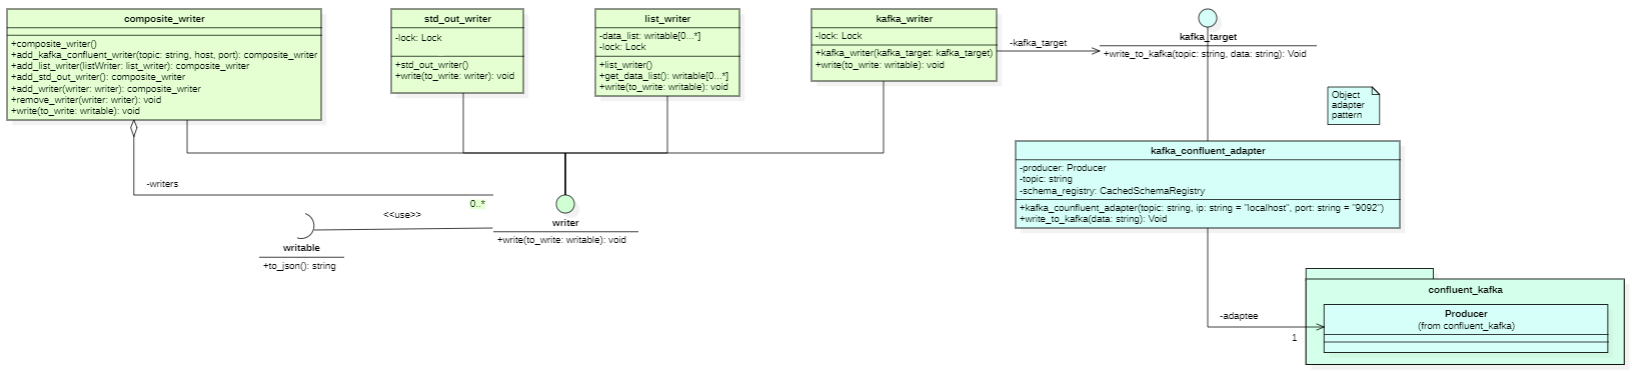
\includegraphics[width=1\textwidth]{../Images/SpecificaTecnica/writerModule.PNG}
    \caption{Modulo Writer - InnovaCity}
    \label{fig: healthModelloWriter}
\end{figure}
Il modulo Writer è il medesimo descritto in \ref{sec:writersModule} e viene nella sua totalità riutilizzato per la scrittura dei punteggi di salute calcolati.
Non viene riportata la strategia di scrittura su di una lista poichè non ne è stato ritenuto necessario l'utilizzo.

\paragraph*{Classi, interfacce metodi e attributi}
Tutte le informazioni sono già state esposte in: \ref{sec:writersModule}.

\subsubsection{Modulo Threading/Scheduling}
\begin{figure}[H]
    \centering
    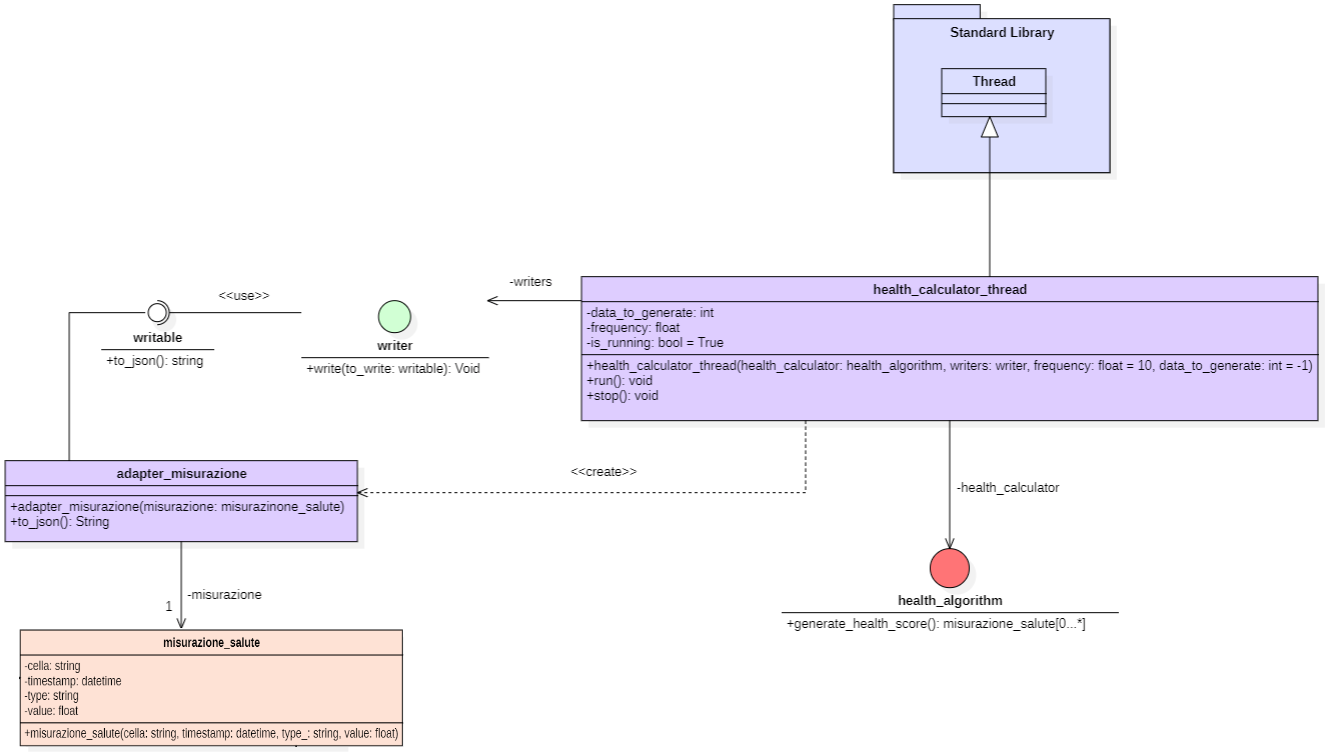
\includegraphics[width=1\textwidth]{../Images/SpecificaTecnica/healthThreading.PNG}
    \caption{Modulo Threading/Scheduling health Model - InnovaCity}
    \label{fig: threadHealth}
\end{figure}

Questo modulo si occupa di integrare la logica di Scheduling e Threading per il calcolo periodico del punteggio di salute della città e quella di scrittura/invio di \textit{writable}. In particolare, fornisce un'implementazione di un thread che, a intervalli regolari, richiama il calcolo del punteggio di salute della città. Successivamente, utilizzando il modulo \textit{Writer}, adatta le misurazioni di salute ottenute all'interfaccia \textit{writable} per inviare i dati al topic \textit{Kafka}\textsubscript{\textit{G}} e/o stamparli su terminale. Pertanto, questo modulo è utilizzatore del modello per il calcolo del punteggio di salute e del modulo di \textit{Writer}.
Il modulo è stato progettato per rispettare il Dependecy Inversion Principle \textit{(DIP)}, di conseguenza sia i moduli di alto livello che quelli di basso livello dipendono da astrazioni (interfacce o classi astratte).

In sintesi, il modulo:
    \begin{enumerate}
        \item Richiama l'algoritmo per calcolo del punteggio di salute della città a intervalli regolari;
        \item Scrive il risultato ottenuto sul topic \textit{Kafka}\textsubscript{\textit{G}}\textsubscript{\textit{G}} dedicato.
    \end{enumerate}

\paragraph*{Classi, interfacce, metodi e attributi}
\begin{itemize}
    \item{\textbf{Classe: \textit{health\_calculator\_thread}}}
    \begin{itemize}
        \item\textbf{Attributi:}
        \begin{itemize}
            \item \textbf{health\_calculator: health\_algorithm [private]} - Un implementatazione dell'interfaccia \textit{health\_algorithm}, ovvero una strategia per il calcolo del punteggio di salute;
            \item \textbf{frequency: float [private]} - La frequenza con cui il thread genera nuovi punteggi di salute;
            \item \textbf{is\_running: bool [private]} - Un flag che indica se il thread è in esecuzione;
            \item \textbf{data\_to\_generate: int [private]} - Il numero di misurazioni di salute da generare;
            \item \textbf{writers: writer [private]} - Un oggetto che implementa la classe \textit{writer}. (Singolo scrittore o albero, Composite \textit{pattern}\textsubscript{\textit{G}})
        \end{itemize}
        \item \textbf{Metodi: }
        \begin{itemize}
            \item \textbf{run(): None [public]} - Esegue il thread, generando nuovi punteggi di salute ad una certa frequenza;
            \item \textbf{stop(): None [public]} - Ferma l'esecuzione del thread.
        \end{itemize}
        \item\textbf{Note:}
        \begin{itemize}
            \item La classe estende la classe \textit{threading.Thread};
            \item Se \textit{data\_to\_generate} è minore di zero, genera misurazioni di salute finchè il thread non viene interroto dall'esterno;
            \item   Grazie al \textit{pattern}\textsubscript{\textit{G}} \textit{Strategy} è possibile cambiare agevolmente l'algoritmo volto al calcolo del punteggio di salute della città.
        \end{itemize}
    \end{itemize}
    \item{\textbf{Classe: \textit{adapter\_misurazione}}}
    \begin{itemize}
        \item \textbf{Metodi: }
        \begin{itemize}
            \item \textbf{to\_json(): String [public]} - Ritorna una stringa JSON compatibile con lo schema richiesto nello Schema Registry per le misurazione di salute.
        \end{itemize}
        \item\textbf{Note:}
        \begin{itemize}
            \item Rappresenta il componente adapter del \textit{pattern}\textsubscript{\textit{G}} \textit{Object adapter};
            \item L'adapter adatta le misurazioni di salute ottenute dall'algoritmo di calcolo del punteggio di salute all'interfaccia \textit{writable} per l'invio al topic \textit{Kafka}\textsubscript{\textit{G}}\textsubscript{\textit{G}}.
        \end{itemize}
    \end{itemize}
\end{itemize}

\subsubsection{Modulo Processing}
\begin{figure}[H]
    \centering
    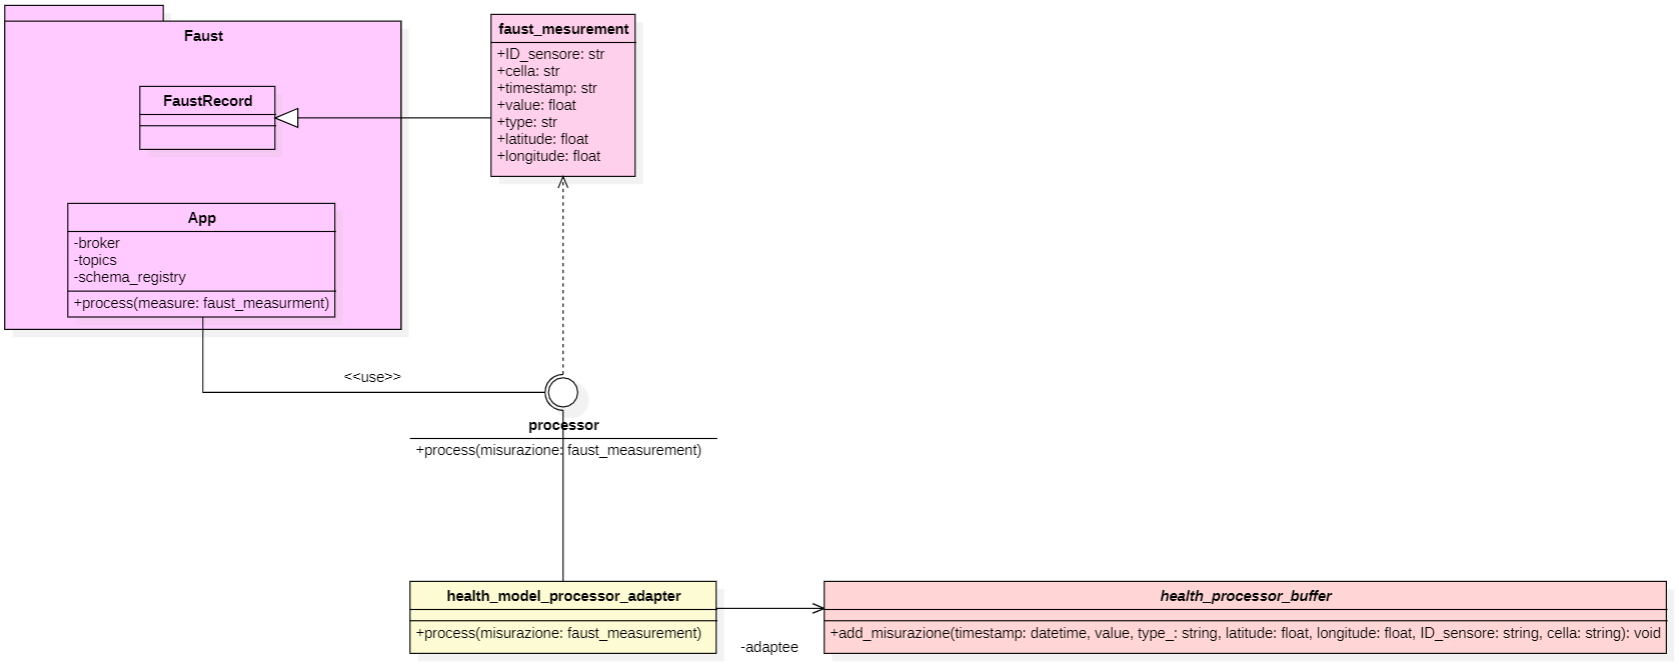
\includegraphics[width=1\textwidth]{../Images/SpecificaTecnica/processorFaust.PNG}
    \caption{Modulo Processing - InnovaCity}
    \label{fig: processHealth}
\end{figure}
Al fine garantire un'interfaccia uniforme delle operazioni di elaborazione dei dati provenienti da \textit{Kafka}\textsubscript{\textit{G}}\textsubscript{\textit{G}} tramite Faust e per stabilire un canale di comunicazione con il modello per il calcolo del punteggio di salute, viene sviluppato il modulo di Processing. Il modulo offre l'interfaccia target denominata \textit{processor}, e un suo adapter denominato \textit{health\_model\_processor\_adapter} per l'invio delle misurazioni al modello per il calcolo del punteggio di salute.

\paragraph*{Design Pattern Object Adapter}
Nel contesto dell'applicazione Faust, all'interno del ruolo svolto dagli agenti, ogni volta che una misurazione viene ricevuta, viene invocato il metodo \textit{process()} dell'implementazione dell'interfaccia \textit{processor} denominata \textit{health\_model\_processor\_adapter}.

In particolare, \textit{health\_model\_processor\_adapter} adatta la classe astratta \textit{health\_processor\_buffer}, che rappresenta un buffer di misurazioni utilizzato per eseguire il calcolo periodico del punteggio di salute della città, all'interfaccia \textit{processor}.

Questo \textit{pattern}\textsubscript{\textit{G}} consente di definire dei contratti per le logiche di elaborazione e di rendere il modello indipendente dall'implementazione specifica dell'applicazione Faust. Allo stesso tempo, facilita la sostituzione dell'operazione di elaborazione eseguita su ogni misurazione dagli agenti grazie al contratto definito nell'interfaccia \textit{processor}.
\paragraph*{Classi, interfacce, metodi e attributi}
\begin{itemize}
    \item{\textbf{Interfaccia: \textit{processor}}}
    \begin{itemize}
    \item\textbf{Metodi: }
    \begin{itemize}
        \item \textbf{process(misurazione: faust\_measurement): None [public, abstract]} - Metodo astratto che deve essere implementato nelle sottoclassi per effettuare elaborazioni di una misurazione.
    \end{itemize}
    \item\textbf{Note:}
        \begin{itemize}
            \item  Le sottoclassi devono implementare il metodo astratto \textit{process()} definendo la propria operazione da effettuare su ogni misurazione ricevuta dai topic di iscrizione;
            \item Rappresenta la componente "Target" del \textit{pattern}\textsubscript{\textit{G}} \textit{Object Adapter};
            \item L'interfaccia è stata progettata per garantire e rappresentare un contratto uniforme per i metodi di elaborazione dei dati provenienti da \textit{Kafka}\textsubscript{\textit{G}}\textsubscript{\textit{G}} tramite Faust;
            \item Gli agenti in ascolto sul topic utilizzeranno un implementatazione di \textit{processor} per effettuare l'elaborazione delle misurazioni ottenute.
        \end{itemize}
    \end{itemize}
    \item{\textbf{Classe: \textit{faust\_measurement}}}
    \begin{itemize}
    \item\textbf{Attributi:}
        \begin{itemize}
        \item \textbf{timestamp: str} - Il timestamp della misurazione;
        \item \textbf{value: float} - Il valore della misurazione;
        \item \textbf{type: str} - Il tipo della misurazione;
        \item \textbf{latitude: float} - La latitudine della misurazione;
        \item \textbf{longitude: float} - La longitudine della misurazione;
        \item \textbf{ID\_sensore: str} - L'\textit{ID}\textsubscript{\textit{G}} del \textit{sensore}\textsubscript{\textit{G}} che ha effettuato la misurazione;
        \item \textbf{cella: str} - La cella in cui è stata effettuata la misurazione.
    \end{itemize}
    \item\textbf{Note:}
        \begin{itemize}
            \item La classe \textit{faust\_measurement} definita eridatando da \textit{faust.Record} rappresenta un singolo record di misurazione proveniente da un \textit{sensore}\textsubscript{\textit{G}} consumata da un'applicazione Faust;
            \item Faust si occupa automaticamente della conversione dei dati in formato JSON sulla base degli attributi definiti, facilitando la ricezione e la deserializzazione dei dati nei topic \textit{Kafka}\textsubscript{\textit{G}}\textsubscript{\textit{G}};
            \item \textbf{In sintesi:}
            Questa classe viene utilizzata in un'applicazione Faust per definire il tipo dei dati attesi nei topic \textit{Kafka}\textsubscript{\textit{G}}\textsubscript{\textit{G}} di interesse. I dati provenienti dai sensori, contenenti timestamp, valore, tipo, coordinate geografiche, identificativo del \textit{sensore}\textsubscript{\textit{G}} e eventuale cella di appartenenza, verranno convertiti in oggetti di tipo \textit{faust\_measurement} prima di essere elaborati dall'applicazione.
        \end{itemize}
    \end{itemize}
    \item{\textbf{Classe: \textit{health\_model\_processor\_adapter}}}
    \begin{itemize}
    \item\textbf{Attributi:}
        \begin{itemize}
        \item \textbf{health\_calculator: health\_processor\_buffer} - Un implementazione della classe astratta \textit{health\_processor\_buffer}.
    \end{itemize}
    \item \textbf{Metodi: }
    \begin{itemize}
        \item \textbf{process(misurazione: faust\_measurement): None [public, async]} - Aggiunge la misurazione ad un implementazione della classe astratta \textit{health\_processor\_buffer} adattando un oggetto di tipo \textit{faust\_measurement} alla porta di accesso fornita da \textit{health\_processor\_buffer} per l'elaborazione volta al calcolo del punteggio di salute.
    \end{itemize}
    \item\textbf{Note:}
        \begin{itemize}
            \item La classe implementa l'interfaccia \textit{processor} ed implementa il metodo astratto \textit{process()} per aggiungere/adattare la misurazione del tipo \textit{faust\_measurement} ad un implementatazione di \textit{health\_processor\_buffer};
            \item Rappresenta la componente "Adapter" del \textit{pattern}\textsubscript{\textit{G}} \textit{Object Adapter};
            \item Il fine è adattare la classe astratta \textit{health\_processor\_buffer} o più in generale il modello per il calcolo del punteggio di salute, all'interfaccia \textit{processor} per l'elaborazione delle misurazioni provenienti dai topic \textit{Kafka}\textsubscript{\textit{G}}\textsubscript{\textit{G}} e consumate dagli agenti Faust.
        \end{itemize}
    \end{itemize}
\end{itemize}